
\documentclass[letterpaper,hide notes,xcolor={table,svgnames},pdftex]{beamer}
\def\showexamples{t}


%\usepackage[svgnames]{xcolor}

%% Demo talk
%\documentclass[letterpaper,notes=show]{beamer}

\usecolortheme{crane}
\setbeamertemplate{navigation symbols}{}

\usetheme{MyPittsburgh}
%\usetheme{Frankfurt}

%\usepackage{tipa}

\usepackage{hyperref}
\usepackage{graphicx,xspace}
\usepackage[normalem]{ulem}

\newcommand\SF[1]{$\bigstar$\footnote{SF: #1}}



\newcounter{tmpnumSlide}
\newcounter{tmpnumNote}

% old question code
%\newcommand\question[1]{{$\bigstar$ \small \onlySlide{2}{#1}}}
% \newcommand\nquestion[1]{\ifdefined \presentationonly \textcircled{?} \fi \note{\par{\Large \textbf{?}} #1}}
% \newcommand\nanswer[1]{\note{\par{\Large \textbf{A}} #1}}


 \newcommand\mnote[1]{%
   \addtocounter{tmpnumSlide}{1}
   \ifdefined\showcues {~\tiny\fbox{\arabic{tmpnumSlide}}}\fi
   \note{\setlength{\parskip}{1ex}\addtocounter{tmpnumNote}{1}\textbf{\Large \arabic{tmpnumNote}:} {#1\par}}}

\newcommand\mmnote[1]{\note{\setlength{\parskip}{1ex}#1\par}}

%\newcommand\mnote[2][]{\ifdefined\handoutwithnotes {~\tiny\fbox{#1}}\fi
% \note{\setlength{\parskip}{1ex}\textbf{\Large #1:} #2\par}}

%\newcommand\mnote[2][]{{\tiny\fbox{#1}} \note{\setlength{\parskip}{1ex}\textbf{\Large #1:} #2\par}}

\newcommand\mquestion[2]{{~\color{red}\fbox{?}}\note{\setlength{\parskip}{1ex}\par{\Large \textbf{?}} #1} \note{\setlength{\parskip}{1ex}\par{\Large \textbf{A}} #2\par}\ifdefined \presentationonly \pause \fi}

\newcommand\blackboard[1]{%
\ifdefined   \showblackboard
  {#1}
  \else {\begin{center} \fbox{\colorbox{blue!30}{%
         \begin{minipage}{.95\linewidth}%
           \hspace{\stretch{1}} Some space intentionally left blank; done at the blackboard.%
         \end{minipage}}}\end{center}}%
         \fi%
}



%\newcommand\q{\tikz \node[thick,color=black,shape=circle]{?};}
%\newcommand\q{\ifdefined \presentationonly \textcircled{?} \fi}

\usepackage{listings}
\lstset{%
  keywordstyle=\bfseries,
  aboveskip=15pt,
  belowskip=15pt,
  captionpos=b,
  identifierstyle=\ttfamily,
  escapeinside={(*@}{@*)},
  stringstyle=\ttfamiliy,
  frame=lines,
  numbers=left, basicstyle=\scriptsize, numberstyle=\tiny, stepnumber=0, numbersep=2pt}

\usepackage{siunitx}
\newcommand\sius[1]{\num[group-separator = {,}]{#1}\si{\micro\second}}
\newcommand\sims[1]{\num[group-separator = {,}]{#1}\si{\milli\second}}
\newcommand\sins[1]{\num[group-separator = {,}]{#1}\si{\nano\second}}
\sisetup{group-separator = {,}, group-digits = true}

%% -------------------- tikz --------------------
\usepackage{tikz}
\usetikzlibrary{positioning}
\usetikzlibrary{arrows,backgrounds,automata,decorations.shapes,decorations.pathmorphing,decorations.markings,decorations.text}

\tikzstyle{place}=[circle,draw=blue!50,fill=blue!20,thick, inner sep=0pt,minimum size=6mm]
\tikzstyle{transition}=[rectangle,draw=black!50,fill=black!20,thick, inner sep=0pt,minimum size=4mm]

\tikzstyle{block}=[rectangle,draw=black, thick, inner sep=5pt]
\tikzstyle{bullet}=[circle,draw=black, fill=black, thin, inner sep=2pt]

\tikzstyle{pre}=[<-,shorten <=1pt,>=stealth',semithick]
\tikzstyle{post}=[->,shorten >=1pt,>=stealth',semithick]
\tikzstyle{bi}=[<->,shorten >=1pt,shorten <=1pt, >=stealth',semithick]

\tikzstyle{mut}=[-,>=stealth',semithick]

\tikzstyle{treereset}=[dashed,->, shorten >=1pt,>=stealth',thin]

\usepackage{ifmtarg}
\usepackage{xifthen}
\makeatletter
% new counter to now which frame it is within the sequence
\newcounter{multiframecounter}
% initialize buffer for previously used frame title
\gdef\lastframetitle{\textit{undefined}}
% new environment for a multi-frame
\newenvironment{multiframe}[1][]{%
\ifthenelse{\isempty{#1}}{%
% if no frame title was set via optional parameter,
% only increase sequence counter by 1
\addtocounter{multiframecounter}{1}%
}{%
% new frame title has been provided, thus
% reset sequence counter to 1 and buffer frame title for later use
\setcounter{multiframecounter}{1}%
\gdef\lastframetitle{#1}%
}%
% start conventional frame environment and
% automatically set frame title followed by sequence counter
\begin{frame}%
\frametitle{\lastframetitle~{\normalfont(\arabic{multiframecounter})}}%
}{%
\end{frame}%
}
\makeatother

\makeatletter
\newdimen\tu@tmpa%
\newdimen\ydiffl%
\newdimen\xdiffl%
\newcommand\ydiff[2]{%
    \coordinate (tmpnamea) at (#1);%
    \coordinate (tmpnameb) at (#2);%
    \pgfextracty{\tu@tmpa}{\pgfpointanchor{tmpnamea}{center}}%
    \pgfextracty{\ydiffl}{\pgfpointanchor{tmpnameb}{center}}%
    \advance\ydiffl by -\tu@tmpa%
}
\newcommand\xdiff[2]{%
    \coordinate (tmpnamea) at (#1);%
    \coordinate (tmpnameb) at (#2);%
    \pgfextractx{\tu@tmpa}{\pgfpointanchor{tmpnamea}{center}}%
    \pgfextractx{\xdiffl}{\pgfpointanchor{tmpnameb}{center}}%
    \advance\xdiffl by -\tu@tmpa%
}
\makeatother
\newcommand{\copyrightbox}[3][r]{%
\begin{tikzpicture}%
\node[inner sep=0pt,minimum size=2em](ciimage){#2};
\usefont{OT1}{phv}{n}{n}\fontsize{4}{4}\selectfont
\ydiff{ciimage.south}{ciimage.north}
\xdiff{ciimage.west}{ciimage.east}
\ifthenelse{\equal{#1}{r}}{%
\node[inner sep=0pt,right=1ex of ciimage.south east,anchor=north west,rotate=90]%
{\raggedleft\color{black!50}\parbox{\the\ydiffl}{\raggedright{}#3}};%
}{%
\ifthenelse{\equal{#1}{l}}{%
\node[inner sep=0pt,right=1ex of ciimage.south west,anchor=south west,rotate=90]%
{\raggedleft\color{black!50}\parbox{\the\ydiffl}{\raggedright{}#3}};%
}{%
\node[inner sep=0pt,below=1ex of ciimage.south west,anchor=north west]%
{\raggedleft\color{black!50}\parbox{\the\xdiffl}{\raggedright{}#3}};%
}
}
\end{tikzpicture}
}


%% --------------------

%\usepackage[excludeor]{everyhook}
%\PushPreHook{par}{\setbox0=\lastbox\llap{MUH}}\box0}

%\vspace*{\stretch{1}

%\setbox0=\lastbox \llap{\textbullet\enskip}\box0}

\setlength{\parskip}{\fill}

\newcommand\noskips{\setlength{\parskip}{1ex}}
\newcommand\doskips{\setlength{\parskip}{\fill}}

\newcommand\xx{\par\vspace*{\stretch{1}}\par}
\newcommand\xxs{\par\vspace*{2ex}\par}
\newcommand\tuple[1]{\langle #1 \rangle}
\newcommand\code[1]{{\sf \footnotesize #1}}
\newcommand\ex[1]{\uline{Example:} \ifdefined \presentationonly \pause \fi
  \ifdefined\showexamples#1\xspace\else{\uline{\hspace*{2cm}}}\fi}

\newcommand\ceil[1]{\lceil #1 \rceil}


\AtBeginSection[]
{
   \begin{frame}
       \frametitle{Outline}
       \tableofcontents[currentsection]
   \end{frame}
}



\pgfdeclarelayer{edgelayer}
\pgfdeclarelayer{nodelayer}
\pgfsetlayers{edgelayer,nodelayer,main}

\tikzstyle{none}=[inner sep=0pt]
\tikzstyle{rn}=[circle,fill=Red,draw=Black,line width=0.8 pt]
\tikzstyle{gn}=[circle,fill=Lime,draw=Black,line width=0.8 pt]
\tikzstyle{yn}=[circle,fill=Yellow,draw=Black,line width=0.8 pt]
\tikzstyle{empty}=[circle,fill=White,draw=Black]
\tikzstyle{bw} = [rectangle, draw, fill=blue!20, 
    text width=4em, text centered, rounded corners, minimum height=2em]
    
    \newcommand{\CcNote}[1]{% longname
	This work is licensed under the \textit{Creative Commons #1 3.0 License}.%
}
\newcommand{\CcImageBy}[1]{%
	\includegraphics[scale=#1]{creative_commons/cc_by_30.pdf}%
}
\newcommand{\CcImageSa}[1]{%
	\includegraphics[scale=#1]{creative_commons/cc_sa_30.pdf}%
}
\newcommand{\CcImageNc}[1]{%
	\includegraphics[scale=#1]{creative_commons/cc_nc_30.pdf}%
}
\newcommand{\CcGroupBySa}[2]{% zoom, gap
	\CcImageBy{#1}\hspace*{#2}\CcImageNc{#1}\hspace*{#2}\CcImageSa{#1}%
}
\newcommand{\CcLongnameByNcSa}{Attribution-NonCommercial-ShareAlike}

\newenvironment{changemargin}[1]{% 
  \begin{list}{}{% 
    \setlength{\topsep}{0pt}% 
    \setlength{\leftmargin}{#1}% 
    \setlength{\rightmargin}{1em}
    \setlength{\listparindent}{\parindent}% 
    \setlength{\itemindent}{\parindent}% 
    \setlength{\parsep}{\parskip}% 
  }% 
  \item[]}{\end{list}} 




\title{Lecture 18 --- Software Requirements \& Specifications}

\author{Jeff Zarnett \\ \small \texttt{jzarnett@uwaterloo.ca}}
\institute{Department of Electrical and Computer Engineering \\[-1ex]
  University of Waterloo}
\date{\today}


\begin{document}

\begin{frame}
  \titlepage
\end{frame}

\begin{frame}
\frametitle{What are Software Requirements?}

\begin{changemargin}{1cm}

Something that a piece of software is expected to do.

Do not describe how the software should do it.

They can be formal or informal.

\end{changemargin}
\end{frame}

\begin{frame}
\frametitle{Why Create Requirements?}

\begin{changemargin}{1cm}

Creating requirements doesn't seem like an XP activity...

It's necessary to have goals for development.

\end{changemargin}
\end{frame}


\begin{frame}
\frametitle{Types of Requirements}

\begin{changemargin}{1cm}

\begin{enumerate}
	\item Functional Requirements
	\item Non-Functional Requirements
	\item Constraints
\end{enumerate}

Imagine we are making a piece of software for the university so student grades can be entered quickly and easily.

\end{changemargin}
\end{frame}

\begin{frame}
\frametitle{Functional Requirements}
	Functional: something the software does - a function or task.
\end{frame}

\begin{frame}
\frametitle{Functional Requirements}

\begin{changemargin}{1cm}

\begin{itemize}
	\item Professors must be able to input grades.
	\item Professors must be able to update grades once entered.
	\item The system must compute class averages.
	\item Administrators must be able to search for a student's history.
\end{itemize}

\end{changemargin}
\end{frame}

\begin{frame}
\frametitle{Non-Functional Requirements}
	Non-Functional: describe the behaviour of the software.
\end{frame}

\begin{frame}
\frametitle{Non-Functional Requirements}

\begin{changemargin}{1cm}

\begin{itemize}
	\item Professors should be easily able to learn the system.
	\item A student may not see the grades of other students.
	\item A record search must take less than five seconds.
	\item The system downtime must be less than eight hours per month.
\end{itemize}

\end{changemargin}
\end{frame}


\begin{frame}
\frametitle{Constraints}
	Constraints: a specialized type of non-functional requirement that restricts the design or implementation of the system.
\end{frame}

\begin{frame}
\frametitle{Constraints}

\begin{changemargin}{1cm}

\begin{itemize}
	\item The server must run on Linux.
	\item The database must be MySQL.
	\item The server must be implemented using C++.
\end{itemize}

\end{changemargin}
\end{frame}

\begin{frame}
\frametitle{Categorizing Requirements}

\begin{changemargin}{1cm}

It's not always obvious whether a requirement is functional or non-functional. \mnote{he important thing to remember is that a functional requirement is a task the software does, and a non-functional requirement is a quality of the system.}\\
Example: Security \mnote{Security, phrased broadly, is a non-functional requirement. However, the ability for administrators to lock a compromised account is a functional requirement.}

Sometimes we have ``mixed'' requirements.\\
Example: ``The user must be able to search for music on his phone and see results within 10 seconds''. \mnote{This might be fine in your document, but it is important to know that this encompasses a functional component (being able to search) and a non-functional component (results within 10s).}

\end{changemargin}
\end{frame}


\begin{frame}
\frametitle{Controversy about Requirements}

\begin{changemargin}{1cm}

If a system is designed to search songs on your phone, and the search takes one full week to complete...

\mnote{There is some further controversy on whether some software requirements are truly meaningful without associated non-functional requirements. If a system is designed to search songs on your phone, and the search takes one full week to complete, the functional requirement is technically satisfied, but the system is not very useful...}

\end{changemargin}
\end{frame}


\begin{frame}
	\frametitle{Stories}
	\begin{changemargin}{1cm}
		Behaviour Driven Development features \alert{Stories}.
		
		Story describes requirement in a natural way for all parties.
		
		Helps everyone have a common definition of ``done''.
		
		How much detail to include? When to split a story up?
		
	\end{changemargin}
\end{frame}

\begin{frame}
	\frametitle{Story Template}
	\begin{changemargin}{1cm}
	
	Narrative:\\
	As a [role]\\
	I want [feature]\\
	So that [benefit]\\~\\

	Acceptance Criteria: (presented as Scenarios)

	Scenario 1: Title\\
	Given [context]\\
	  And [some more context]...\\
	When  [event]\\
	Then  [outcome]\\
	  And [another outcome]...\\

	Scenario 2: ...
	
	\end{changemargin}
\end{frame}

\begin{frame}
	\frametitle{Stories: Title}
	\begin{changemargin}{1cm}
		Title should give a summary of user behaviour.
		
		Specific is better than vague:\\
		``Module X Behaviour'' vs ``User Prints Invoice''
		
		
	\end{changemargin}
\end{frame}

\begin{frame}
	\frametitle{Stories: Narrative}
	\begin{changemargin}{1cm}
		Answers to questions:
		
		Who will interact with the system? $\rightarrow$ Role.
		
		What to implement? $\rightarrow$ Feature.
		
		Why do this? $\rightarrow$ Benefit. \mnote{The ``why'' of the story is especially important; if you have no answer (or a bad answer like ``because the old system did this''), then you may not have to implement this feature at all.}
		
		
	\end{changemargin}
\end{frame}

\begin{frame}
	\frametitle{Stories: Scenarios}
	\begin{changemargin}{1cm}
		Scenario Title says what is different.
		
		Three elements: \\
		\hfill Given (Context), When (Event), and Then (Outcome).
	
		How many scenarios is too many?		
		
	\end{changemargin}
\end{frame}


\begin{frame}
	\frametitle{Stories: Example Title}
	\begin{changemargin}{1cm}
	Obligatory Automatic Teller Machine (ATM) example.\\
		\hfill ...All discussions of Software Requirements need one.
		
	Title: ``Account Holder Withdraws Cash''
				
	\end{changemargin}
\end{frame}

\begin{frame}
	\frametitle{Stories: Example Narrative}
	\begin{changemargin}{1cm}
	
	As an Account Holder (Role)\\
I want to withdraw cash from an ATM (Feature)\\
So that I can get money when the bank is closed (Benefit)
					
	\end{changemargin}
\end{frame}


\begin{frame}
	\frametitle{Stories: Example Scenario}
	\begin{changemargin}{1cm}
	
Scenario 1: Account has sufficient funds

Given the account balance is \$100\\
 And the card is valid\\
 And the machine contains enough money\\
When the Account Holder requests \$20\\
Then the ATM should dispense \$20\\
 And the account balance should be \$80\\
 And the card should be returned
					
	\end{changemargin}
\end{frame}

\begin{frame}
	\frametitle{Stories: Example Scenario}
	\begin{changemargin}{1cm}
	
Scenario 2: Account has insufficient funds

Given the account balance is \$10\\
 And the card is valid\\
 And the machine contains enough money\\
When the Account Holder requests \$20\\
Then the ATM should not dispense any money\\
 And the ATM should say there are insufficient funds\\
 And the account balance should be \$10\\
 And the card should be returned
					
	\end{changemargin}
\end{frame}

\begin{frame}
	\frametitle{Stories: Example Scenario}
	\begin{changemargin}{1cm}
	
Scenario 3: Card has been disabled

Given the card is disabled\\
When the Account Holder requests \$20\\
Then the ATM should retain the card\\
And the ATM should say the card has been retained
					
	\end{changemargin}
\end{frame}

\begin{frame}
	\frametitle{Stories: Example Scenario}
	\begin{changemargin}{1cm}
	
Scenario 4: The ATM has insufficient funds...

There is no limit to the number of scenarios in a story.\\
\hfill But at some point it makes sense to split it up.

	\end{changemargin}
\end{frame}


\begin{frame}
	\frametitle{Stories: Splitting Up}
	\begin{changemargin}{1cm}
	
	One possible decomposition of the example story:
	
\begin{itemize}
	\item Account holder withdraws cash\\
	\quad(assumptions: ATM is working, card is valid)
	\item Account holder wants to withdraw cash from broken ATM\\
	\quad(assumptions: ATM is malfunctioning, card is valid)
	\item Account holder wants to withdraw cash with invalid card\\
	\quad(assumptions: ATM is working, card is invalid)
\end{itemize}

	\end{changemargin}
\end{frame}



\begin{frame}
\frametitle{Gathering Software Requirements}

\begin{changemargin}{1cm}

Software requirements come from somewhere; we create them.

Use requirements to get customer input into the system.

\end{changemargin}
\end{frame}

\begin{frame}
\frametitle{How NOT to Gather Requirements}

\vspace{4cm}

\begin{quote}
	\textit{If I had asked people what they wanted, they would have said faster horses.}
\end{quote}
\hfill Henry Ford (possibly).

\mnote{The fact is that customers do not know what they want, and this goes double for customers who are non-technical. For the most part, users are unable to imagine anything other than a marginally better version of a system they have already worked with}

\mnote{If you ignore this, the likely outcome is that you will create a piece of software the the users will not accept or cannot use. This is not to say that user input is irrelevant, but it is only one piece of the puzzle.}

\end{frame}


\begin{frame}
\frametitle{How to Get User Input}

\begin{changemargin}{1cm}

\begin{enumerate}
	\item Meet with a focus group
	\item Follow users in their workflow
	\item Brainstorming.
\end{enumerate}

Remember: what you get from customers is not requirements; it's data.

\end{changemargin}
\end{frame}


\begin{frame}
\frametitle{Gathering Requirements}

\begin{changemargin}{1cm}

No matter how diligent you are, there will be incorrect, missing, and superfluous requirements. 

Plan accordingly!

\end{changemargin}
\end{frame}


\begin{frame}
	
	
	\vspace{8em}
	
	\begin{block}
	 {\huge Case Study: Satellite Tracking Software }\mnote{In the other part of this lecture, we're going to take a look at a real-world case study relating to embedded systems. Let's examine the case WCDE-00087-01 - developing software for the Canadian Space Agency. We won't repeat the content of that PDF, but the background information will be helpful, so hopefully everyone read it.}
	\end{block}
	
\end{frame}

\begin{frame}
	\frametitle{Case Study: Satellite Tracking Software}
	

	Imagine we are working at the Canadian Space Agency.
	
	We are on the Telemetry, Tracking, and Control (TT\&C) team.
	
	TT\&C team: ensure communication between satellites and Canadian ground stations

	
\end{frame}

\begin{frame}
	\frametitle{Case Study: Satellite Tracking Software}
	
	\begin{center}
	Video: Satellites 101
	\end{center}
	
\end{frame}


\begin{frame}
	\frametitle{Case Study: Satellite Tracking Software}
	
	\begin{changemargin}{1cm}
	Information from the satellite:
	\begin{itemize}
	\item Status of the spacecraft (resources, attitude, operation, health)
	\item Scientific data and images
	\item Orbit and timing data for ground navigation
	\item Tracking object locations
	\end{itemize}
	
	\mnote{Why do we need to track satellites? To communicate with the satellite, as well as observe and control its functions from the ground.}
	
	\end{changemargin}
	
\end{frame}


\begin{frame}
	\frametitle{Case Study: Satellite Tracking Software}
	
	\begin{center}
	Video: Real time satellite in Google Earth
	\end{center}
	
\end{frame}


\begin{frame}
	\frametitle{Case Study: Satellite Tracking Software}
	
	\begin{changemargin}{1cm}
		Satellite Hardware:
		\begin{itemize}
		\item Main antenna
		\item Signal modulation and demodulation equipment
		\item Sensors and transducers
		\item Central computer
	\end{itemize}	
    \end{changemargin}
\end{frame}

\begin{frame}
	\frametitle{Case Study: Satellite Tracking Software}
	
	\begin{changemargin}{1cm}
	Tracking software uses a \alert{mathematical model} of the orbit.
	
	The model takes as input the \alert{current state} of the satellite.
	
	Using this data and the model, the software predicts the \alert{future state} of the satellite.
	
    \end{changemargin}
\end{frame}


\begin{frame}
	\frametitle{Case Study: Satellite Tracking Software}
	
	\begin{center}
	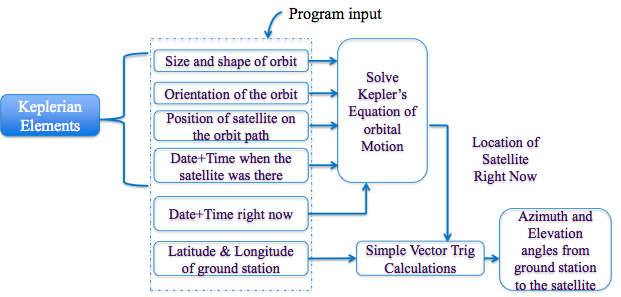
\includegraphics[width=1.25\textheight]{images/casestudysw.png}
	\end{center}
    
\end{frame}

\begin{frame}
	\frametitle{Case Study: Satellite Tracking Software}
	
\begin{center}
	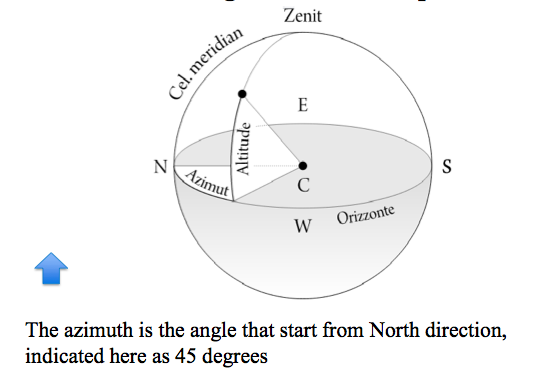
\includegraphics[width=\textheight]{images/azimuth.png}
\end{center}

{\small Note that ``Zenit'' = Zenith, ``Azimut'' = Azimuth, ``Orizzonte'' = Horizon, and ``Cel. meridian'' = Celestial Meridian}
    
\end{frame}



\begin{frame}
	\frametitle{Case Study: Satellite Tracking Software}
	
	\begin{center}
	Video: Satellite Orbit Path
	\end{center}
	
\end{frame}

\begin{frame}
	\frametitle{Case Study: Satellite Tracking Software}
		\begin{changemargin}{1cm}
	From the background, what are some shortcomings in the existing CSA software? \mnote{ask students for their observations from the background material}\vspace{2em}
		\end{changemargin}
\end{frame}

\begin{frame}
	\frametitle{Case Study: Satellite Tracking Software}
	
	\begin{changemargin}{1cm}
	Shortcomings in the existing CSA software:
	\begin{itemize}
		\item Code outdated
		\item Source code was unavailable
		\item Library was a licensed product (license fees)
		\item Did not respond well when called by multiple programs
	\end{itemize}
	\end{changemargin}
			
\end{frame}


\begin{frame}
	\frametitle{Case Study: Satellite Tracking Software}
	
	\begin{center}
	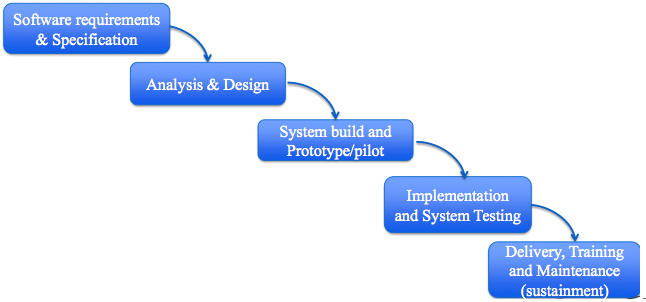
\includegraphics[width=1.25\textheight]{images/casestudywf.png}
	\end{center}
	
	\mnote{Ask why author chose this. My own guess is... the author doesn't know there are other options.}
    
\end{frame}

\begin{frame}
	\frametitle{Case Study: Satellite Tracking Software}
	
	\begin{changemargin}{1cm}
 	What are some 
	\begin{itemize}
		\item Functional Requirements
		\item Non-Functional Requirements
		\item Constraints
	\end{itemize}
	
	of this system? We don't need specific numbers, but try to cover all the areas.
	
	Discuss for a few minutes; then we'll discuss as a class.
	\end{changemargin}
			
	\mnote{Case study answers include: accuracy, reliability, data format, multiple apps to use the software, execution speed, extensibility}
			
\end{frame}


\begin{frame}
\frametitle{Specifications}

~\\~\\~\\~\\
\begin{quote}
	\textit{... specs are like flossing: everybody knows they should be writing them, but nobody does.}
\end{quote}
\hfill Joel Spolsky 

\end{frame}

\begin{frame}
\frametitle{Specifications}
	\begin{changemargin}{1cm}
	Based on software requirements, describe how the software will meet them.
	
	Now it's time to design the program. \mnote{The specification is based on the requirements, and explains in detail how the software will meet the goals set by the requirements. Or, to put it more simply, creating the specification makes you sit down and design the program.}
	
	\end{changemargin}
\end{frame}


\begin{frame}
\frametitle{Specification Motivation}
	\begin{changemargin}{1cm}
		Why not just start coding?
		
		It's faster to change a line of text in a spec than rewrite code. \mnote{ No matter how fast you are at developing software, changing the text ``file uploads take place synchronously and block the UI'' to ``file uploads take place asynchronously and do not block the UI'' takes a tiny fraction of the time it would take to make those changes in the software.}
		
		Communication between different parties:
		\begin{itemize}
			\item Developers \mnote{Developers will have a clear idea of not just what is to be done, but also how it should be done}
			\item QA \mnote{can be used by QA to develop tests}
			\item Marketing \mnote{so they know what to sell}
			\item Technical Writers \mnote{so they can make the manuals / guides}
			\item Customers \mnote{So they know what they're getting}
		\end{itemize}
			
		Scheduling \& Planning. \mnote{Having designed the software in detail, you will have a good basis for the schedule. We'll discuss scheduling and planning in another upcoming lecture.}
			
	\end{changemargin}
\end{frame}

\begin{frame}
\frametitle{Without a Spec}
	\begin{changemargin}{1cm}
		
		Most of the communication still takes place, but inefficiently. \mnote{lots of e-mails and meetings and so on while people try to figure things out}
		
		People will get out of sync.
		
		More chance of an error or wasted effort.
					
	\end{changemargin}
\end{frame}

\begin{frame}
\frametitle{Writing a Specification}
	Goal: describe how the product works from a user perspective. \mnote{features, menus, dialogs, user interfaces, etc}
	
	It will never be complete and perfect. Update as required.
	
\end{frame}

\begin{frame}
\frametitle{Writing a Specification}

	\begin{changemargin}{1cm}
	Start with the requirements.
	
	We should be able to examine the requirements and identify which sections of the specification fulfill that requirement.

	Traceability of requirements. \mnote{Later on, during software testing and verification, it will be possible to trace the requirements from the requirements document, through the design documents, and into the verification results. Tracing requirements ensures that all requirements are met, and will make it easier to demonstrate to the customers, management, etc that this is the case.}

	\end{changemargin}
\end{frame}


\begin{frame}
\frametitle{Writing a Specification}

	\begin{changemargin}{1cm}
		Design should be user-focused.
		
		Create a scenario about how a user will use the system.
		
		Example: professor is ready to enter grades. \mnote{The professor first prepares the grades, then logs into the system, navigates to the grade entry screen, selects the class, and then enters the grades next to each student number.}
		
		More detail and realism results in a better specification.
		
	\end{changemargin}
\end{frame}


\begin{frame}
\frametitle{Writing a Specification}

	\begin{changemargin}{1cm}
		It's all about the details.
		
		Describe what should happen whether things go right or wrong.
		
		You may spend more time describing error handling.
		
	\end{changemargin}
\end{frame}

\begin{frame}
\frametitle{Specification: Printing}
		
		\begin{enumerate}
			\item No printers are configured.
			\item Multiple printers are configured, but no default is set.
			\item The data is in colour but the default printer can only print black and white.
			\item The print processor encountered an error.
			\item The print job was sent, but the printer is out of paper or ink.
			\item The printer memory is insufficient to handle the print job.
			\item The print job was sent and is now in the print queue.
			\item The print job completed successfully.
		\end{enumerate}
		\mnote{This is not an exhaustive list. The correct response to each situation depends on the system in question, but the specification should have an answer for each.}
				
\end{frame}

\begin{frame}
\frametitle{Writing a Specification}

	\begin{changemargin}{1cm}
		Sometimes, nothing \emph{should} happen. \mnote{Sometimes, that answer might be ``nothing happens'', and that's fine; document, however, that nothing happening is the expected behaviour.}
		
	Scenario not described in the spec? Add it. \mnote{Your judgement may tell you what the correct solution is, but you should nevertheless update the specification.}
	
	Update the specification regularly.\\
	Otherwise it becomes useless if not misleading. \mnote{Much like cleaning a home, if you do a little bit every day the amount of work seems manageable; if you ignore it for a long time then it becomes a full day of work.}
		
	\end{changemargin}
\end{frame}

\begin{frame}
\frametitle{A Collection of Stories}
\begin{changemargin}{1cm}
Remember stories?

The specification can be a collection of stories.

Just assemble all the stories.

\end{changemargin}
\end{frame}


\begin{frame}
\frametitle{Writing a Specification}

	\begin{changemargin}{1cm}
		Specs are hard to write as a team.
		
		If it's too large, split it up so one person is responsible for some sections.
		
		Co-ordinate to keep them consistent.
		
	\end{changemargin}
\end{frame}


\begin{frame}
\frametitle{Specification Tips}

	\begin{changemargin}{1cm}
		Tip 1: Write simply.
		
		Don't write ``utilize'' instead of ``use''.
		
		`~The query must complete within 10 seconds''\\vs.\\ ``It is an absolute requirement that under all circumstances that should a user elect to execute a query on the system, the maximum upper bound on execution time thereof is 10 seconds''
		
				
	\end{changemargin}
\end{frame}




\begin{frame}
\frametitle{Specification Tips}

	\begin{changemargin}{1cm}
		Tip 2: Review \& Reread.
		
		Should be an ongoing process.
		
		Rewrite parts that are hard to understand.		
				
	\end{changemargin}
\end{frame}


\begin{frame}
\frametitle{Specification Tips}

	\begin{changemargin}{1cm}
		Tip 3: Avoid Templates.
		
		Might sound like a good idea, but overly formal...
		
		People already hate doing specs - don't make it worse.		
				
	\end{changemargin}
\end{frame}

\begin{frame}
\frametitle{Specification Tips}

	\begin{changemargin}{1cm}
		Tip 4: Don't be boring.
		
		Funny is one way, but I don't recommend it.
		
		If your spec is an insomnia cure...
				
	\end{changemargin}
\end{frame}

\begin{frame}
\frametitle{Specification Example}

	\begin{changemargin}{1cm}
			Our example will be \emph{Fog Creek Copilot}\\
			\quad Providing tech support over the internet.
			
			Called in internal documentation ``Aardvark''.
			
	\end{changemargin}
\end{frame}

\begin{frame}
\frametitle{Copilot/Aardvark Overview}

	\begin{changemargin}{1cm}
	
	``Aardvark allows people to help their friends, relatives, and customers with their computer problems by temporarily taking over their computers over the Internet.'' 
	
	\end{changemargin}
\end{frame}


\begin{frame}
\frametitle{Copilot/Aardvark Major Features}

	\begin{changemargin}{1cm}
	
	\begin{itemize}
	\item Easy to get started: \begin{itemize} \item No software needs to be permanently installed; \item Simple fast payment and no commitment \end{itemize}
	\item Version 1.0 is Windows only and requires a reasonable broadband connection.
	\item Blasts through all firewalls as long as outbound connections on port 443 are allowed.
	\item Secure (hopefully).
\end{itemize}

	\end{changemargin}
\end{frame}

\begin{frame}
\frametitle{Copilot/Aardvark: Making Changes}

	\begin{changemargin}{1cm}
\begin{quote}
\textit{When I wrote the first draft of this spec, I had a more complicated flowchart that assumed that either party (helper or victim) could initiate the process. This became extremely complicated and convoluted for various reasons. As I worked through the screens that would be needed to allow either party to initiate the process, I realized that Aardvark would be just as useful, and radically simpler, if the helper was required to start the whole process. Making this change in the spec took an hour or two. If we had made this change in code, it would have added weeks to the schedule.}
\end{quote}
	\end{changemargin}
\end{frame}

\begin{frame}
\frametitle{Copilot/Aardvark: UI Examples}


\begin{center}
	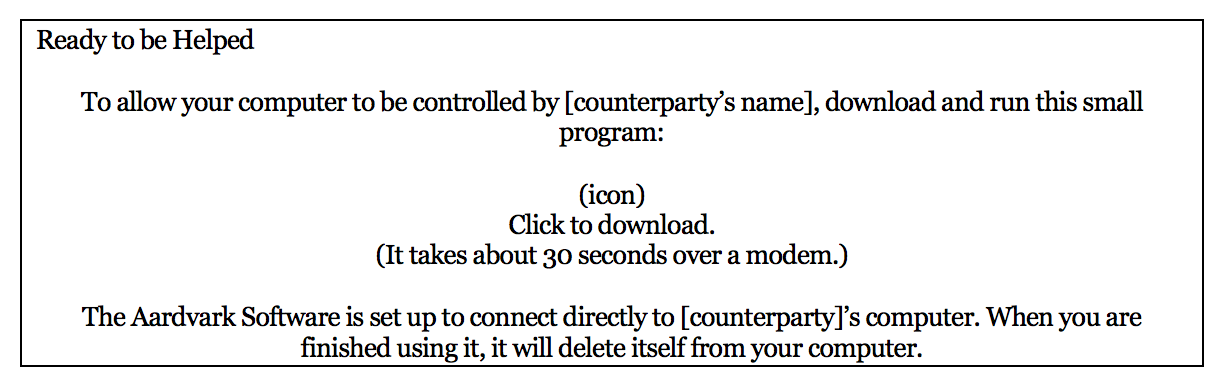
\includegraphics[width=\textwidth]{images/aardvarkui.png}
\end{center}

\end{frame}

\begin{frame}
\frametitle{Copilot/Aardvark Future Features}

	\begin{changemargin}{1cm}
	
\begin{itemize}
	\item Ability to transfer files between helper and victim, possibly with drag and drop.
	\item Chat features, either voice or IM style.
\end{itemize}

	\end{changemargin}
\end{frame}

\begin{frame}
\frametitle{Copilot/Aardvark: Pictures = 1000 Words}


\begin{center}
	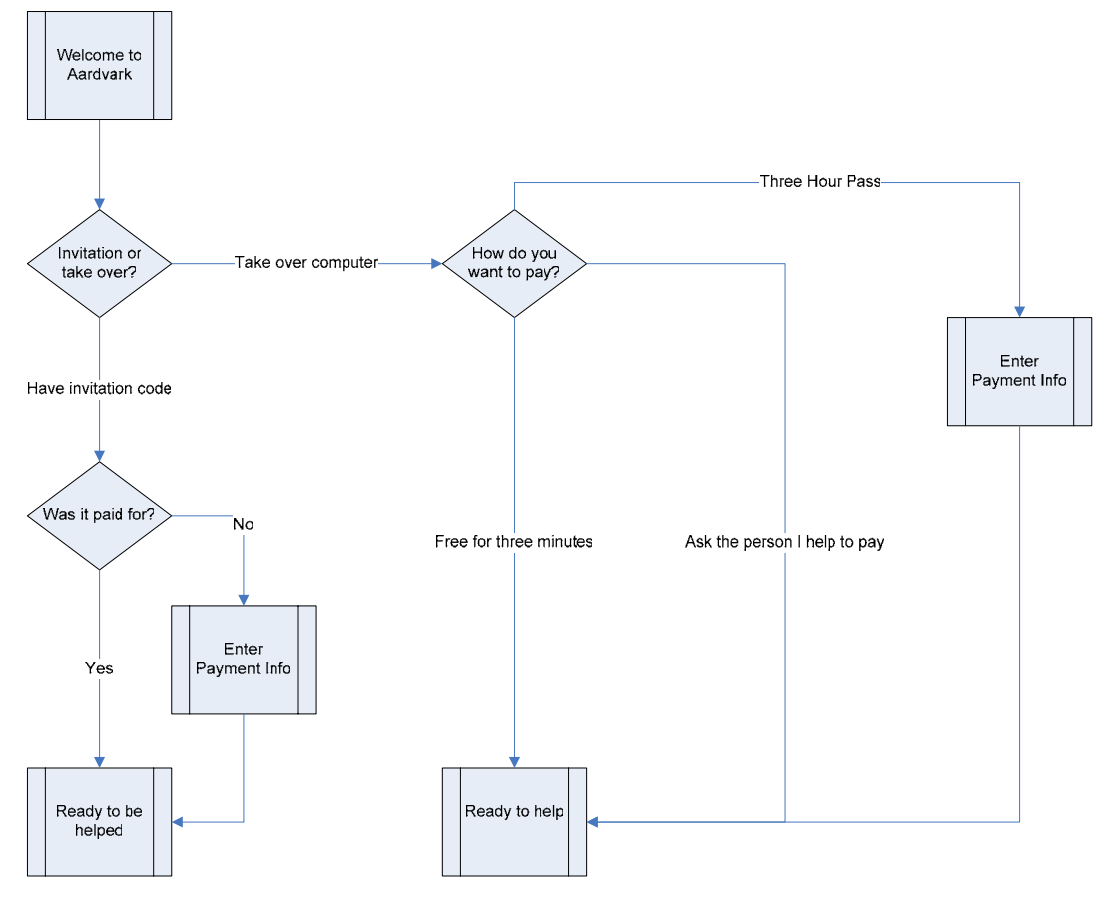
\includegraphics[width=0.75\textwidth]{images/aardvarksite.png}
\end{center}


\end{frame}


\end{document}
